Die Kernpunkte der Auswertung des zweiten Algorithmus unterscheiden sich etwas von den Zielen der anderen Auswertung. Zum einen soll hier auch wieder eine Bewertung hinsichtlich der Art und Höhe der möglichen Optimierungen stattfinden. Im Unterschied zur anderen Umsetzung sollen die Lösungsverfahren des TSP theoretisch die gleiche, beste Lösung ermitteln. Ein erstes Ziel wäre es also alle Verfahren bezüglich ihrer Nutzbarkeit und Praxisuntauglichkeit zu bewerten, um alle anschließenden Tests dann nur mit dem daraus bestimmten, besten Verfahren durchzuführen.

\subsubsection{Testszenario 1: Bestimmung der Parameter für das Simulated Annealing Verfahren}

Bevor die Verfahren gegeneinander bewertet werden können, müssen zunächst einmal die besten Werte für das Simulated Annealing Verfahren gefunden werden. Die variablen Paramater sind dabei: startingTemperature, coolingRate und numberOfIterations. Ziel dieses Testszenarions ist es, diese Parameter zu variieren und so die bestmöglichen Eingabewerte für den gegebenen Anwendungsfall zu finden. In der Testklasse \textit{SimAParameterTest} wurden dafür die im Folgenden beschriebenen Abläufe implementiert, mit dem R-Skript \textit{tspSimAParameter} wurden die Ergebnisse ausgewertet, sowie die hier dargestellten Graphen erzeugt.

Schaut man sich die Implementierung des Algorithmus genauer an, so ist numberOfIterations einfach die maximale Anzahl von Schleifendurchläufen und sozusagen eine Begrenzung, damit der Algorithmus im schlimmsten Fall nicht ewig läuft. Um diesen Parameter sinnvoll einschätzen zu können, wurden alle folgenden Testdurchläufe mit dem Wert Integer.MAX\_VALUE durchgeführt, somit wird es so viele Schleifendurchläufe geben, wie es braucht. Die benötigte Anzahl wird hier jeweils in die CSV-Datei mit den Ergebnisdatensätzen übernommen. Somit können hier im Nachhinein die höchsten benötigten Werte abgelesen werden, um eine sinnvolle Einschätzung der notwendigen Iterationen zu erhalten und für den Worst-Case ein mit Spielraum versehenes Limit gesetzt werden. Hauptsächlich abhängig ist das Ergebnis des Algorithmus also von startingTemperature und coolingRate. Die startingTemperature darf sich dabei in einem theoretischen Bereich von >0,1 und unendlich bewegen. Die coolingRate muss für sinnvolle Ergebnisse >0 und <1 sein. Um hier einen Gesamteindruck der Auswirkung dieser beiden Parameter auf das Ergebnis zu erhalten, sollen diese beiden Variablen systematisch in Schleifen variiert werden und jeweils die Kosten berechnet werden. Es entsteht somit ein dreidimensionaler Datensatz der Kosten in Abhängigkeit von startingTemperature und coolingRate. Für das Gesamtbild wird ein zufälliger, aber fester Graph generiert. Mit diesem wird der SimA Algorithmus mit jeder Kombination von startingTemperature und coolingRate einmal ausgeführt. Um das Verhalten über verschiedenen Graphen zeigen zu können, wird dieser gesamte Prozess mit 100 verschiedenen Graphen ausgeführt. In ersten, losen Test hat sich gezeigt, dass der wirklich interessante Teil bei startingTemperature etwa im Intervall [1;100] liegt und die coolingRate etwa bei [0.9;1[. Um die Übersichtlichkeit zu wahren und die Ausführungsdauer der Tests einzuschränken, wurden die Tests deshalb auf diese Intervalle konzentriert. Die startingTemperature wurde dabei in Schritten von 1 erhöht, die coolingRate jeweils um 0,001.

Nachfolgende Graphen (Abb. \ref{fig:evalSimAParams}) zeigen das Ergebnis dieser Auswertung. Gezeigt werden dabei in einem farblichen Verlauf die durchschnittlichen Kosten über aus den 100 Durchläufen mit verschiedenen Graphen zu einem Paar aus startingTemperature und coolingRate. Die grünen Bereiche zeigen dabei, wo die Kosten tendenziell am geringsten sind und die roten Bereiche repräsentieren die höchsten Kosten. Da auch die Größe des zu bearbeitenden Graphen einen Einfluss hat, wurde dieser gesamte Test mit Graphen mit den Größen 10, 20, 50 und 100 Knoten wiederholt. Mit Blick auf die zu erwartenden LKW \todo{in konzeption/Anforderungen erwähnen?!} wird dies wird voraussichtlich der Bereich sein, in dem der Algorithmus zum Lösen des TSP verwendet wird.

\begin{figure}[H]
\centering
\begin{subfigure}{.495\textwidth}
  \centering
  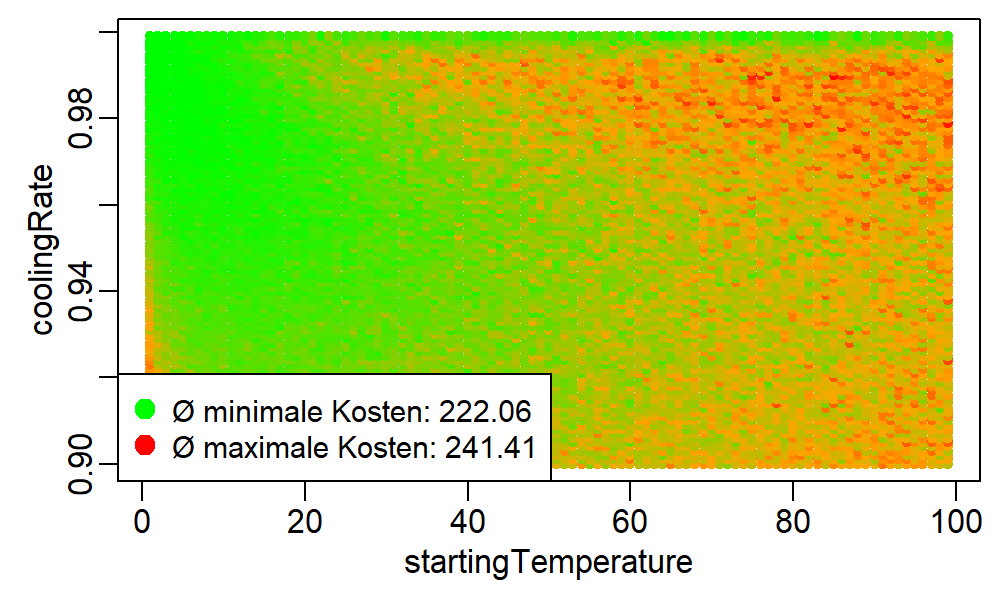
\includegraphics[width=\linewidth]{images/graphs/tspSimAParameter10.png}
  \caption{Graph mit 10 Knoten}
  \label{fig:esp1}
\end{subfigure}
\begin{subfigure}{.495\textwidth}
  \centering
  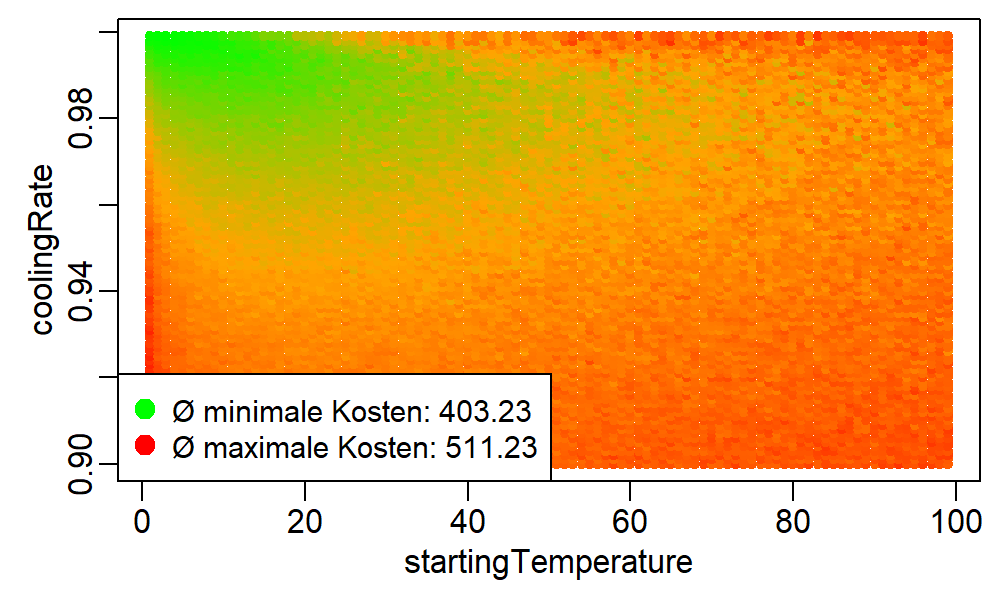
\includegraphics[width=\linewidth]{images/graphs/tspSimAParameter20.png}
  \caption{Graph mit 20 Knoten}
  \label{fig:esp2}
\end{subfigure}

\begin{subfigure}{.495\textwidth}
  \centering
  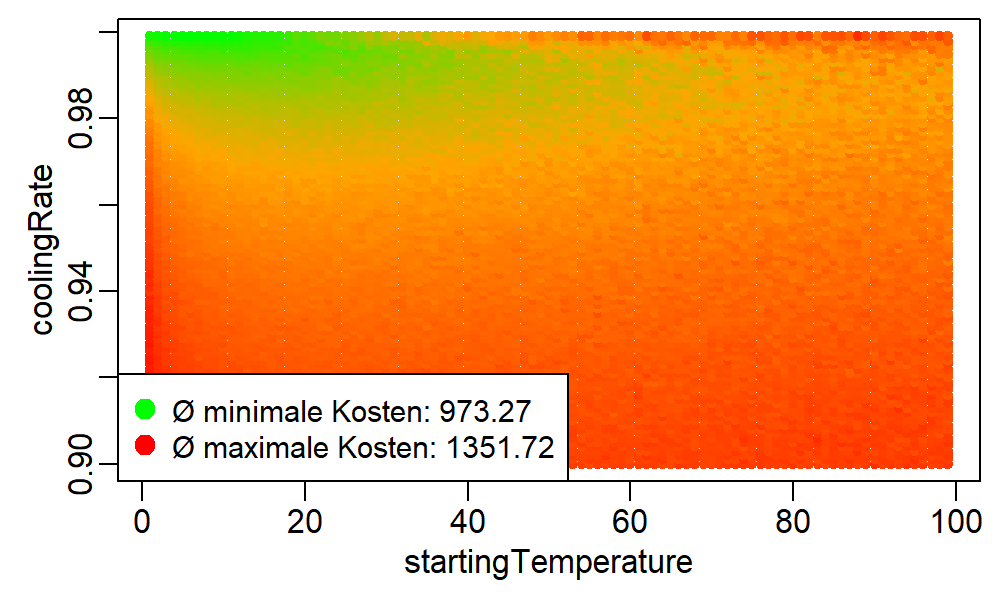
\includegraphics[width=\linewidth]{images/graphs/tspSimAParameter50.png}
  \caption{Graph mit 50 Knoten}
  \label{fig:esp3}
\end{subfigure}
\begin{subfigure}{.495\textwidth}
  \centering
  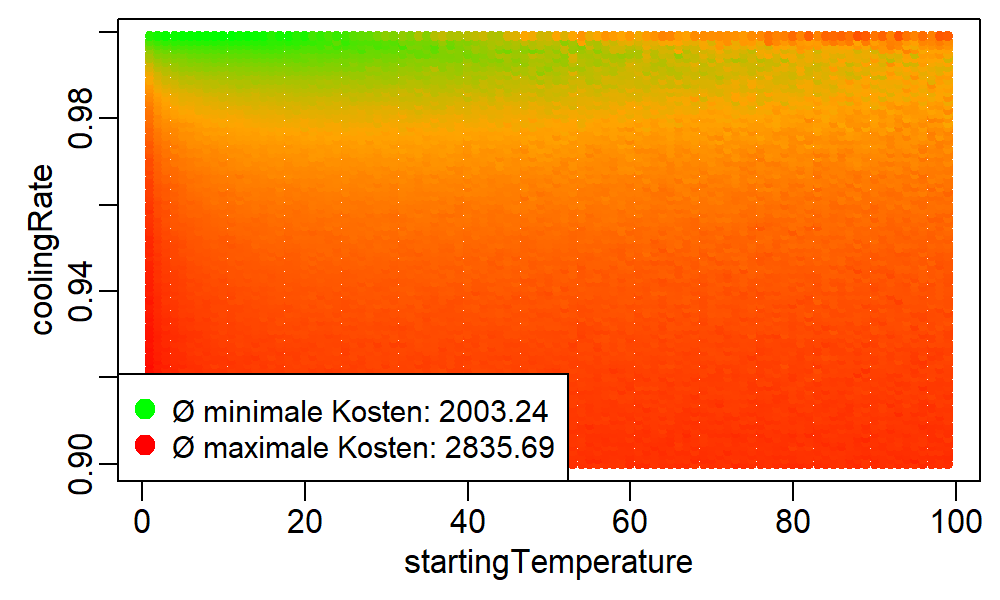
\includegraphics[width=\linewidth]{images/graphs/tspSimAParameter100.png}
  \caption{Graph mit 100 Knoten}
  \label{fig:esp4}
\end{subfigure}
\caption{Simualted Annealing mit variierten Parametern}
\label{fig:evalSimAParams}
\end{figure}

Für die besten Werte der Parameter lassen sich daraus nun einige Schlussfolgerungen ziehen. Zur benötigten Anzahl von Iterationen lässt sich aus den resultierenden Wertetabellen ablesen, dass diese relativ stark schwankt, das Maximum liegt in diesem Beispiel aber bei 6895\todo{finalen Wert eintragen}. Selbst wenn man die Grenze für den Worst-Case nun extrem großzügig auf beispielsweise 100.000 setzt, ist dies immer noch ein Wert, der in der Berechnung problemlos handhabbar ist. Selbst diese Zahl von Iterationen sollte nicht für nennenswert hohe Ausführungszeiten sorgen. Diese Höhe von Iterationen wird aber wenn überhaupt ohnehin extrem selten erreicht.

Die dargestellten Graphen lassen nun eine gute Einschätzung zu, wie die beiden weiteren Parameter zu wählen sind. Grundsätzlich werden sich dabei keine exakten Werte bestimmen lassen, da es sich hier immer noch um Zufallswerte handelt, für die immer etwas andere Parameter optimal wären. Gerade bei geringer Anzahl von Knoten ist zu erkennen, dass die Kosten auch bei nah aneinander liegenden Punkten deutliche Schwankungen haben, da sehr unterschiedlich farbige Punkte nah beieinander liegen und kein gleichmäßiger Verlauf entsteht. Dennoch lässt sich eine sehr gute Tendenz erkennen, bei welcher Kombination von Parametern die Kosten optimal gering werden. Bei geringer Anzahl von Knoten ist die Wahl der Parameter noch nicht ganz so kritisch, hier ist der optimale, grüne Bereich noch relativ groß. Hier würde eine startingTemperature $<$ 50 und eine coolingRate $>$ 0,9 in der Regel schon sehr gute Werte liefern. Mit größerer Anzahl von Knoten wird dieser Bereich deutlich kleiner. Hier sollte vor allem die coolingRate so nah wie möglich an 1 liegen. Gute Werte werden hier tendenziell nur noch bei startingTemperature $<$ 40 und coolingRate $>$ 0,99 erzielt. Die grünen Bereiche der Graphen überschneiden sich allerdings, was sehr gut es, denn gut Werte für 100 Knoten liefern somit auch z.B. bei 10 Knoten ebenfalls gute Ergebnisse. Eine startingTemperature von 15 und eine coolingRate von 0,9995 sollten also gut geeignet sein.

Abschließend wurden die hier ermittelten Werte (numberOfIterations=100.000, startingTemperature=15, coolingRate=0,9995) als Standardwerte in die Variablen der Klasse \textit{SimulatedAnnealingAlgorithm} übernommen. Über in diesen Tests verwendeten Konstruktor können wie bisher variable Werte verwendet werden, werden diese Werte allerdings über den weiteren Konstruktor nicht gesetzt, so werden immer die hier ermittelten, besten Werte verwendet. Alle weiteren Testszenarien arbeiten also dann direkt mit diesen Werten.

\subsubsection{Testszenario 2: Laufzeit und Grenzen}
\todo{Leistungsdaten des Rechners angeben?!}
\todo{Grund für das nicht weiter verfolgen der anderen Verfahren genannet, also warum z.B. nicht mit noch mehr Rechenleistung getestet wurde? -> Zu großer aufwand für absehbar wenig mehr Knoten, SimA bietet mehr Erfolgsaussichten}

Wie schon bei der Implementierung aufgefallen ist, werden insbesondere die exakten Verfahren früher oder später durch ihre Laufzeit bei der Berechnung oder durch ihren Arbeitsspeicherbedarf begrenzt sein. Der nötige Aufwand ist dabei zum bedeutendsten Teil von der Anzahl der Knoten des zu lösenden Graphen abhängig. Um also zunächst die Lösungsverfahren selbst zu bewerten, sind hier noch gar keine Vergleiche und Auswertungen hinsichtlich des eigentlichen Problemszenarios nötig. Viel mehr ist hier die Laufzeit bei der Berechnung der Ergebnisse für die einzelnen Verfahren von Interesse. Aus diesem Grund arbeiten die folgenden Tests, welche in der Testklasse \textit{RunTimeTest} implementiert wurden auch direkt mit den Algorithmus-Klassen, ohne Ladeplätze, Slotlimiterungen o.ä. zu berücksichtigen. Ausgeführt wird also immer jeder Algorithmus einmal mit dem identischen Eingangsgraphen. Dabei wird schrittweise die Anzahl der Knoten erhöht. Für jede Anzahl von Knoten werden dabei 10 Durchläufe mit unterschiedlichen, zufälligen Graphen erzeugt, um sinnvolle Durchschnittswerte und Streuungen bei der Berechnungszeit ermitteln zu können. Da hier keine exakten Ergebnisse, sondern vor allem Größenordnungen interessant sind, reichen hier 10 Wiederholungen. Um die Ausführungszeit darüber hinaus im Rahmen zu halten, wurde ein Begrenzung eingebaut, sodass die Algorithmen für mehr Knoten nicht mehr ausgeführt werden, wenn entweder einmal der Speicherplatz ausgegangen ist oder wenn die Ausführung zu lange gedauert (Limit von 10 Minuten) \todo{Erhöhen für eine Ausführung von 16 Knoten?!} hat. Die Tendenz sollte dann erkennbar sein und eine stunden- oder tagelange Ausführung der Tests ist nicht nötig. Die folgende Auswertung (Tabelle \ref{tab:evalTspRunTime}) wurde durch das R-Skript \textit{tspRunTime.R} berechnet. Als Darstellungsform wurde in diesem Fall eine Tabelle gewählt, da sich die Werte stark voneinander unterscheiden. Die wichtigen Aspekte wären in einem Graphen nicht gut sichtbar.


\begin{table}[H]
    \caption{Durchschnittliche Laufzeiten der Verfahren (Alle Werte in s)}
    \label{tab:evalTspRunTime}
    \centering
    \begin{tabular}{c|c|c|c|c|c|c}
        \textbf{Knoten} & \textbf{Ø SimA} & \textbf{$\sigma$ SimA} & \textbf{Ø BnB} & \textbf{$\sigma$ BnB} & \textbf{Ø RM} & \textbf{$\sigma$ RM} \\\hline\hline
        \csvreader[
            %column count=4,
            %no head,
            %table head=\hline\hline,
            %table head=\textbf{Labels} & \textbf{Labels} & \textbf{Labels} & \textbf{Labels} \\\hline,
            late after line=\\\hline,
            late after last line=\\
        ]
        {files/tspRunTime_out.csv}
        {1=\one, 2=\two, 3=\three, 4=\four, 5=\five, 6=\six, 7=\seven, 8=\eight}
        {\two & \three & \four & \five & \six & \seven & \eight}
    \end{tabular}
\end{table}
\todo{Mit mehr Durchläufen asuführen, sternchen an einfach ausgeführten einfügen}

Sehr deutlich zu erkennen ist, dass der Aufwand zum Lösen des Problems exponentiell mit der Anzahl der Knoten steigt. Insbesondere für das Reduced Matrix und das Branch and Bound Verfahren bedeutet dies, dass der Aufwand ab etwa 10 Knoten merklich höher wird und jeweils bei 13 bzw. 15 Knoten so groß wird, dass dies zumindest für eine größere Zahl von Wiederholungen in dieser Auswertung deutlich zu viel ist. Das Reduced Matrix Verfahren scheitert dabei an einem \glqq{}java.lang.OutOfMemoryError: Java heap space\grqq{} Fehler, welcher zeigt, dass der Arbeitsspeicher der Java VM nicht ausreicht, selbst mit einer Erhöhung auf 8 GB. Die Laufzeit der Berechnung steigt zwar auch erheblich, aber dem ersten Anschein nach nicht so schnell wie im Branch and Bound Verfahren. Hier kostet bereits die Berechnung von 15 Knoten im Durchschnitt ca. 16 Minuten, während es bei 14 Knoten noch ca. 3 Minuten waren. Aus diesem Grund wurden auch die letzten Durchläufe jeweils nur mit einer Wiederholung durchgeführt und bilden somit nur einen Anhaltspunkt der Ausführungszeit, aber keinen sinnvollen Durchschnitt mehr\todo{finaler Stand?}. Bei diesen Verfahren zeigt sich aber auch eine hohe Standardabweichung bei der Ausführungszeit zwischen verschiedenen Durchläufen. Dies dürfte damit zusammenhängen, dass diese Verfahren je nach Eingabewerten unterschiedlich viel Zeit sparen. Das Simulated Annealing Verfahren zeigt dagegen über wesentlich längere Zeit deutlich geringere Ausführungszeiten. Insgesamt ist bei der mehrfachen Ausführung dieser Testklasse sichtbar geworden, dass die Ausführungszeiten auch zwischen diesen Ausführungen schwanken. Dies hat insbesondere beim Branch and Bound Verfahren mit 14 Knoten einen sichtbaren unterschied von einigen Sekunden gemacht. Dies dürfte auch mit der sonstigen Auslastung des Computers im Hintergrund zu tun haben. Eine deutliche Tendenz ist aber sehr klar sichtbar und ändert nichts an den extrem steigenden Zeiten.




\textbf{Qualität der Verfahren}

Gleichzeitig sind die Werte dieses Szenarios ein guter Anhaltspunkt, um die Qualität der Verfahren untereinander zu vergleichen. Insbesondere das Simulated Annealing Verfahren findet nicht unbedingt das beste Ergebnis, sodass hier auch gleichzeitig ein direkter Vergleich stattfinden kann. Als Metrik bietet sich hier die Höhe der Gesamtkosten bzw. der Gesamtzeit des gefundenen Weges durch den Graphen an, da dies auch der Wert ist, nachdem beim TSP optimiert wird. Diese zweite Auswertung (siehe Tabelle \ref{tab:evalTspTotalCost}) wurde mit den identischen CSV-Daten durch das R-Skript \textit{tspTotalCost.R} berechnet. Auch hier wurde die Darstellung in einer Tabelle gewählt, da übereinanderliegende und starkt steigende Werte so deutlich besser sichtbar sind.

\begin{table}[H]
    \caption{Durchschnittliche Kosten der Verfahren (Alle Werte in min)}
    \label{tab:evalTspTotalCost}
    \centering
    \begin{tabular}{c|c|c|c|c|c|c}
        \textbf{Knoten} & \textbf{Ø SimA} & \textbf{$\sigma$ SimA} & \textbf{Ø BnB} & \textbf{$\sigma$ BnB} & \textbf{Ø RM} & \textbf{$\sigma$ RM} \\\hline\hline
        \csvreader[
            late after line=\\\hline,
            late after last line=\\
        ]
        {files/tspRunTime_costOut.csv}
        {1=\one, 2=\two, 3=\three, 4=\four, 5=\five, 6=\six, 7=\seven, 8=\eight}
        {\two & \three & \four & \five & \six & \seven & \eight}
    \end{tabular}
\end{table}
\todo{Mit mehr Durchläufen ausführen, sternchen an einfach ausgeführten einfügen}

\todo{Streuung sinnvoll, da immer andere Graphen?! Oder hier evtl Variationskoeffizient, um relative schwankung darzustellen?}

Erkennbar ist, die exakten Verfahren BnB und RM durchgängig identische Werte liefern. Die Abweichung von RM bei 13 Knoten ist damit zu erklären, dass hier aufgrund vom Speichermangel nicht mehr alle Durchläufe berechnet werden konnten, während es bei BnB ein Durchschnitt aus allen 10 Iterationen ist. Auch das SimA Verfahren zeigt bis 10 Knoten identische Werte. Dies zeigt, dass in diesen Bereichen von allen Verfahren das gleiche und serh wahrscheinlich auch optimale Ergebnis erzielt wurde. Ab 11 Knoten fängt es an, dass die Ergebnisse des SimA Verfahrens etwas schlechter werden, als die höchst wahrscheinlich optimalen Ergebnisse der anderen Verfahren. Aufgrund der bereits erkannten Beschränkungen bezüglich Laufzeit und Speicherbedarf lässt sich diese Tendenz so einfach nicht weiter bestätigen. Dies bestätigt aber auch die Theorie des Simulated Annealing, dass eben in der Regel ein sehr gutes, aber nicht perfektes Ergebnis erzielt wird \todo{Quelle?}. Somit lässt sich vermuten, dass die Ergebnisse auch bei einer sehr viel größeren Zahl von Knoten sehr gut sind.

Insgesamt zeigt sich als großer Vorteil des Simulated Annealing Verfahrens, dass schon mit einfachen Rechen-Ressourcen eine wesentlich höhere Zahl von Knoten, weit über 1000 Knoten möglich ist. Dies übersteigt die hier realistisch zu erwartende Größe von Graphen um ein vielfaches. Insbesondere wenn ein mTSP, also eine Verteilung für mehrere Ladeplätze ermittelt werden soll und somit noch einige Knoten für Ladeplätze verbraucht werden, sind 12-15 Knoten sehr schnell erreicht. Ein sinnvoller Einsatz von Branch and Bound und Reduced Matrix Verfahren ist (in der hier implementierten Variante) also eigentlich nicht möglich. Selbst wenn man die Rechen-Ressourcen deutlich aufstockt, wird der Bedarf weiter exponentiell steigen. Damit ist möglicherweise eine Erhöhung der Knotenanzahl im unteren einstelligen Bereich möglich, eine sinnvoll nutzbare Anzahl wird dies aber höchstwahrscheinlich immer noch nicht. Für die weiteren Tests wird deshalb mit dem Simulated Annealing Verfahren weiter gearbeitet.


\subsubsection{Testszenario 3: Streuung zwischen den Simulated Annealing Durchläufen}

In diesem Szenario geht es darum, wie groß die Streuung der optimierten Kosten beim mehreren Durchläufen des selben Graphen ist. Während vorherigem explorativen Ausprobierens der Verfahren ist aufgefallen, dass sich die Ergebnisse, also die Gesamtkosten zwischen den Durchläufen eines eigentlich identischen Graphen unterscheiden. Dies dürfte aber nur für den Simulated Annealing Ansatz relevant sein, da hier mit gewissen Zufallsprozessen, dem \glqq{}Abkühlungsvorgang\grqq{} gearbeitet wird. Bei den anderen Verfahren ergibt sich immer das beste Ergebnis, bei allerdings höherer Rechenzeit, wie die vorherigen Tests gezeigt haben. Da mit dem Simulated Annealing Verfahren weiter gearbeitet werden soll, soll dieser Umstand an dieser Stelle aber noch einmal genauer untersucht werden.

Das Vorgehen, welches in der Testmethode \textit{spreadTest()} der Testklasse \textit{SimulatedAnnealingTest} implementiert wurde und zur Ermittlung passender Werte dient, ist wie folgt: Die prinzipielle Idee ist es, das Simulated Annealing Verfahren mit dem identischen Eingangsgraphen mehrfach laufen zu lassen. Es wird dabei bei jeden weiteren Durchlauf immer das beste Ergebnis, also die geringsten Durchlaufkosten aller vorherigen Iterationen gespeichert. Die Idee dabei ist, dass man angesichts des geringen Zeitaufwands eines SimA Durchlaufs einfach immer mehrere Durchläufe macht und das insgesamt beste Ergebnis zurück gibt. Um auch hier wieder einen aussagekräftigen Durchschnitt ermitteln zu können, wird das Ganze in einer Schleife mit 100 verschiedenen Graphen durchgeführt. Dargestellt wird immer die prozentuale Abweichung von dem insgesamt für diesen Graphen besten ermittelten Wert, welcher nach Formel \ref{eq:simaResBestCost} berechnet wurde. Diese Darstellung wurde gewählt, da der absolut beste Wert je nach Graphen etwas unterschiedlich ist. In dieser Aufbereitung lässt sich ein besserer Vergleich ziehen. Allerdings ist dieser Wert auch nicht als überhaupt minimal erreichbarer Wert zu verstehen, aber auch bei noch wesentlich mehr Durchläufen bleibt die Kurve nicht konstant bei 0\%, da es sich aber um wenige Fälle und nur noch minimale Verbesserungen handelt, wurde hier der Übersicht halber 70 Durchläufe als Maximum gewählt. Als Größe für den Graphen wurden hier exemplarisch 50 LKW bei 3 Ladeplätzen gewählt, was mit insgesamt 53 Knoten im oberen erwartbaren Bereich liegt, was die potenzielle Größe der Graphen angeht. Je Größer der Graph ist, desto mehr Algorithmus Durchläufe wird es tendenziell benötigen, um das absolut mögliche Minimum zu finden.

\begin{equation} \label{eq:simaResBestCost}
relativ Beste Kosten = \left(\left(\frac{absolut Beste Kosten}{minimale Kosten Der Iteration}\right)*100\right)-100
\end{equation}

\begin{figure}[H]
    \centering
    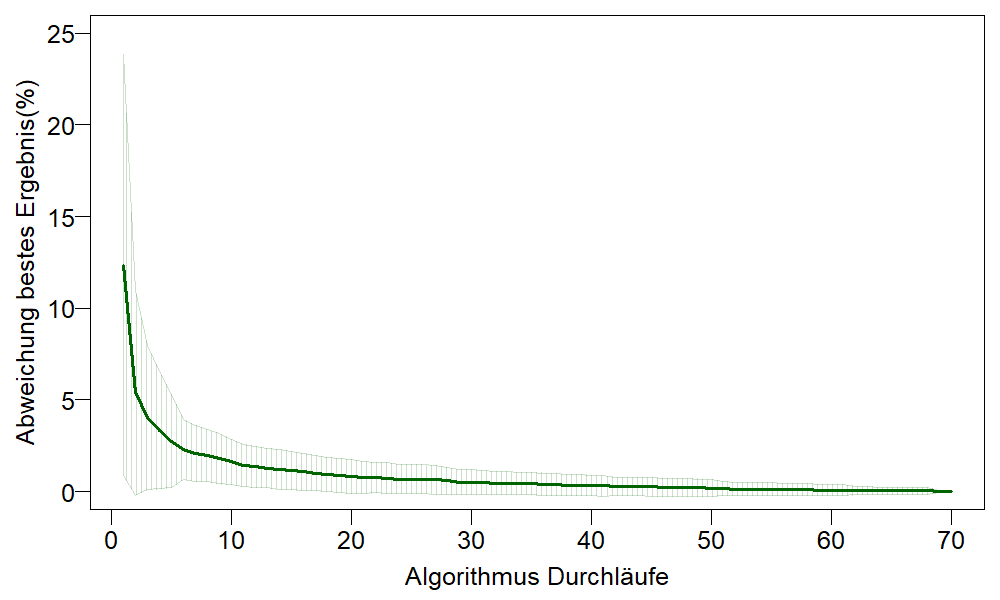
\includegraphics[width=0.7\textwidth]{images/graphs/tspResultSpreadTest.png}
    \caption{Bestes Ergebnis des Simualted Annealing Verfahrens nach mehreren Durchläufen}
    \label{fig:tspEvalSpread}
\end{figure}

\todo{Legende}

In Abbildung \ref{fig:tspEvalSpread} ist erkennbar, dass es zu Beginn mit nur einem einzigen Algorithmuslauf eine sehr große Unsicherheit gibt. Im Durchschnitt ist das Ergebnis etwa 12\% schlechter, als es im besten Fall nach 70 Durchläufen möglich war. Auch die Standardabweichung ist extrem hoch, d.h. es gibt Fälle in denen das Ergebnis nach einem Durchlauf bereits sehr gut ist, in anderen Fällen ist dies da aber noch sehr viel schlechter. Die Kurve sinkt allerdings schon nach wenigen Durchläufen sehr stark. Nach etwa 5 Läufen ist das Ergebnis im Mittel nur noch ca. 3\% schlechter bei auch sehr viel geringerer Streuung. Ab ca. 10 Läufen werden die Ergebnisse auch deutlich langsamer besser.  Für den realen Einsatz des Simulated Annealing Verfahrens lässt sich daraus schlussfolgern, dass eine wiederholte Ausführung zum finden des besten Ergebnisses durchaus sinnvoll ist. Schon eine 5 bis 10-fache Iteration kann die größten Unsicherheiten beseitigen. Angesichts der wirklich sehr geringen Laufzeiten im Millisekunden-Bereich (siehe Tabelle \ref{tab:evalTspRunTime}), kann man sogar über eine wesentlich höhere Zahl von 30 bis 50 oder sogar noch mehr Durchläufen nachdenken. Selbst wenn dann Berechnungszeiten von wenigen Sekunden entstehen, ist dass für den realen Einsatz noch lange kein Problem.


\subsubsection{Testszenario 4: Verbesserung der Abfertigungszeit}

Nachdem nun viel Aufwand in die Bestimmung des besten Lösungsverfahrens sowie in die beste Verwendung der Verfahren geflossen ist, sollen nun Versuche zum eigentlichen Ziel der Optimierung durchgeführt werden. Gearbeitet werden soll dabei, wie in den vorherigen Tests bestimmt wurde, mit dem Simulated Annealing Alogrithmus. Genutzt wird immer das beste Ergebnis aus 50 Durchläufen. Außerdem werden die Buchungen immer auf 3 Ladeplätze aufgeteilt. Interessant ist hier in erster Linie, wie viel sich die gesamte Abfertigungszeit gegenüber dem unoptimierten Ausgangszustand verbessern lässt. Es wird dabei immer die durch den SimA-Algorithmus optimierten Wert mit den unoptimierten Werten verglichen, welche mit aus der Zeitplanung des UnoptimizedAlgorithm ermittelt wurden. Einmal soll das Ganze für einen unbegrenzten Zeitraum simuliert werden. Die gleichen Tests werden aber auch noch einmal für einen begrenzten Slot durchgeführt werden. Interessant sind diese Werte, da dies auch schlussendlich das für den realen Einsatz bedeutende Ergebnis ist. Da die Begrenzung allerdings ein weiterer, auf die eigentliche Optimierung aufbauender Schritt ist, wird hier diese getrennte Betrachtung durchgeführt. Implementiert wurden die Tests in den Testmethoden \textit{test3LoadersBestOf50()} und \textit{test3LoadersBestOf50Limited()} der Testklasse \textit{SimulatedAnnealingTest}. Das R-Skript \textit{tspOptimization.R} diente zur Auswertung.

Im Graphen dargestellt ist zum einen, wie sich die Gesamtzeit verbessert hat, bis alle LKW bearbeitet wurden. Berechnet wurde dieser Wert nach Formel \ref{eq:tspCostSaving}. Zusätzlich ist eine Kurve sichtbar, welche die Verbesserung bei der Zahl der eingeplanten LKW zeigt. Dieser Wert wird über Formel \ref{eq:tspSchedImpr} berechnet. Beide Werte werden prozentual dargestellt, da so ein relativer Vergleich mit steigender Anzahl von LKW Buchungen möglich ist.

\begin{equation} \label{eq:tspSchedImpr}
schedImpr = \dfrac{oScheduledJobs-uScheduledJobs}{uScheduledJobs} * 100
\end{equation}

\begin{equation} \label{eq:tspCostSaving}
costImpr = \dfrac{uCost-oCost}{uCost} * 100
\end{equation}

%\begin{equation} \label{eq:tspTtcSaving}
%ttcSaving = \dfrac{uTimeToComplete-oTimeToComplete}{uTimeToComplete} * 100
%\end{equation}


\begin{figure}[H]
\centering
\begin{subfigure}{.495\textwidth}
  \centering
  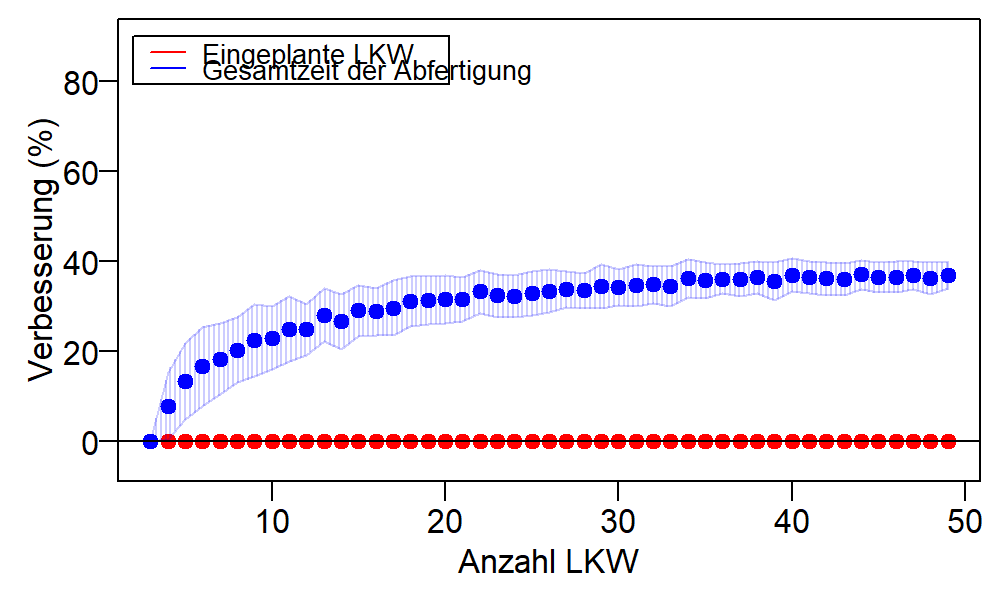
\includegraphics[width=\linewidth]{images/graphs/tspSimulatedAnnealingUnlimited.png}
  \caption{Unbegrenzter Slot}
  \label{fig:etspsimaopt2}
\end{subfigure}
\begin{subfigure}{.495\textwidth}
  \centering
  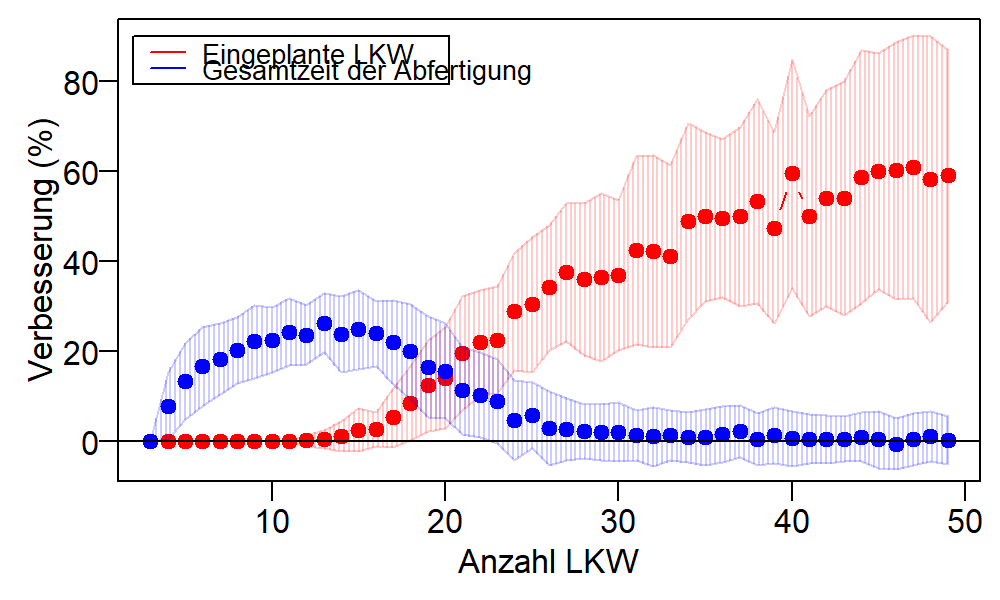
\includegraphics[width=\linewidth]{images/graphs/tspSimulatedAnnealingLimited.png}
  \caption{3 Stunden Slot}
  \label{fig:etspsimaopt2}
\end{subfigure}
\caption{Verbesserung der Abfertigungszeit}
\label{fig:evalTspSimAOpt}
\end{figure}

\todo{Time to complete darstellen?; Punkte weg, nur linie}

Zunächst einmal ist an den Ergebnisgraphen zu erkennen, dass mit dem hier untersuchten Algorithmus definitiv gute Verbesserungen erzielt werden können. Gibt es keine Slotbegrenzung, so können immer alle LKW abgefertigt werden, die rote Linie ist also konstant bei 0, da die Zahl der geplanten LKW in beiden Modellen identisch ist. Die Gesamtzeit, die es braucht, alle LKW zu bearbeiten verbessert sich dagegen. Zunächst einmal steigt diese Verbesserung stark an, sodass bereits bei 10 LKW eine über 20\% kürzere Abfertigungszeit möglich ist. Dann steigt die Verbesserung immer langsamer und nähert sich bis ca. 50 LKW den 40\% an. Die Standardabweichung, also die Streuung der Gesamtabfertigungszeit ist über den gsamten Bereich nicht besonders hoch, verringert sich aber mit streigender Anzahl von LKW noch einmal. Viel interessanter ist allerdings das Verhalten bei begrenztem Slot. Bis ca. 14-15 LKW verhalten sich beide Kurven sehr ähnlich, hier entstehen durch die Slotbegrenzung noch gar keine Einflüsse, im unoptimierten, wie im optimierten Fall können hier noch alle LKW eingeplant werden. Die Verbesserung der Abfertigungszeit erreicht hier auch sein Maximum. Ab dann verbessert sich die Zahl der LKW, welche eingeplant werden können. Im unoptimierten Fall müssen nun langsam die ersten LKW abgewiesen bzw. in andere Slots verschoben werden. Die Zahl der eingeplanten LKW steigt nun sehr stark an und erreicht bei 50 gebuchten LKW knapp 60\% Verbesserung. Allerdings erhöht sich auch die Streuung extrem, d.h. es gibt Fälle in denen deutlich mehr LKW erfolgreich eingeplant werden können, als in anderen. Die Verbesserung der gesamten Abfertigungszeit sinkt ab ca. 15 LKW wieder und nähert sich bei gleichbleibender Streuung der 0 an. Dies liegt daran, dass der Slot in beiden Fällen sehr gut voll ausgelastet wird. Allerdings ist die Zeit pro LKW deutlich geringer, sodass mehr LKW in die gleiche Zeit passen, wie die andere Kurve eben gezeigt hat. 

Insgesamt lässt sich aus diesem Test schlussfolgern, dass mit dem hier getesteten Verfahren durchaus gute Verbesserungen erzielt werden können. Die Höhe der Verbesserung hängt davon ab, wie viele LKW pro Slot gebucht werden dürfen, bzw. ob und in welcher Höhe Überbuchungen erlaubt werden. So hat der Algorithmus mehr Planungsspielraum, es müssten allerdings auch Buchungen auf andere Slots verschoben werden. Um hie die optimale Größe zu finden, wurde das nächste Testszenario durchgeführt.

\subsubsection{Testszenario 5: Verhalten bei Überbuchung}

Wie im vorherigen Szenario festgestellt wurde, hat die Zahl der LKW, welche einen Slot buchen können einen bedeutenden Einfluss auf die Höhe der möglichen Verbesserung. Es stellt sich nun die Frage, ob man eine harte Grenze einführen sollte und keine Buchungen mehr zulässt, wenn die erste Buchung nicht mehr in den Slot passt. Die andere Option wäre es, wie es auch schon für den anderen hier entwickelten Algorithmus empfohlen wurde, eine gewissen Überbuchung zuzulassen. In diesem Fall müssten einige Buchungen zwangsweise im Nachhinein auf spätere Slots verschoben werden. So ergibt sich aber ein noch größerer Spielraum für den Planungsalgorithmus und somit möglicherweise noch weiter verbesserte Abfertigungszeiten. 

Ein entsprechender Testfall wurde in der Testklasse \textit{SimulatedAnnealingTest} in der Methode \textit{test3LoadersBestOf50LimitedOverfill()} implementiert. Der Grundaufbau und die gesammelten Daten sind dabei wie im vorherigen Test. Hier wird allerdings für ein Testreihe die gleiche Liste von Buchungen beibehalten und nur schrittweise eine weitere hinzugefügt. Dies simuliert, dass weitere LKW Fahrer bzw. Speditionen diesen Slot buchen. Dargestellt wird im Auswertungsgraphen dieses mal aber die absolute Zahl von Buchungen, um zeigen zu können, wann nicht mehr alle LKW eingeplant werden können. Eine diagonale Gerade der Steigung 1 zeigt dann des theoretischen Anstieg, ohne begrenzten Slot. Auf einer zweiten y-Achse wird dagegen die Verbesserung der Gesamtkosten aufgetragen, berechnet nach dem gleichen Weg, wie im vorherigen Szenario (siehe Formel \ref{eq:tspCostSaving}).

\begin{figure}[H]
    \centering
    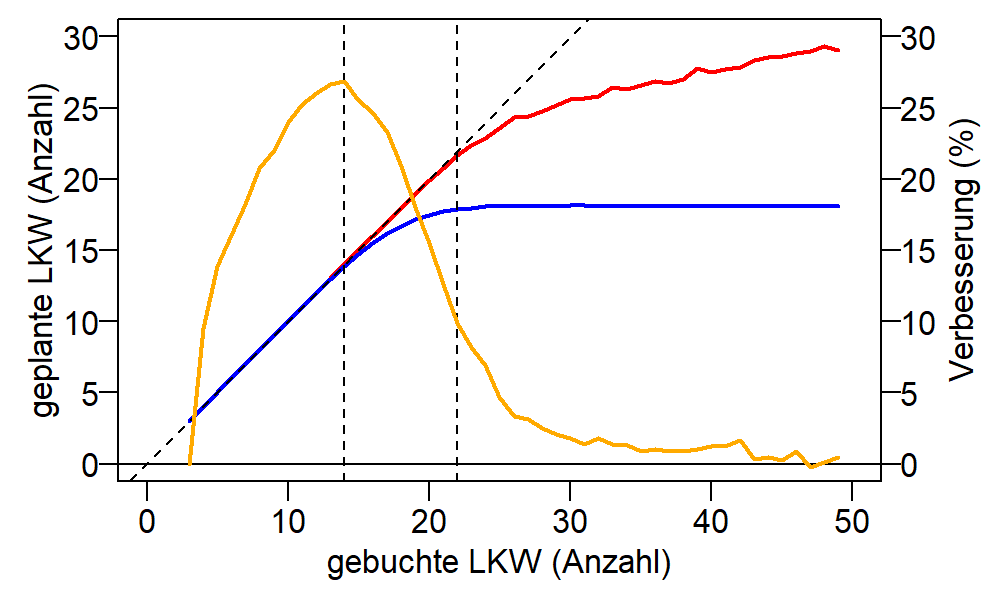
\includegraphics[width=0.7\textwidth]{images/graphs/tspSimALimOverfill.png}
    \caption{Verhalten bei Überbuchung}
    \label{fig:tspEvalOverfill}
\end{figure}

In der Auswertung ist gut zu erkennen, dass selbst bei strikter Begrenzung des Slots eine deutliche Verbesserung möglich ist. Während die blaue Kurve schon bei etwa 14 LKW abfällt und somit zeigt, dass schon nicht immer alle LKW in den Slot passen, fängt die rote, optimierte Kurve erst bei etwa 22 LKW an, langsam abzufallen. Das heißt, selbst wenn bei der Buchung nur so viele LKW zugelassen werden, wie auch in den Slot passen, lassen sich im Durchschnitt schon etwa 8 LKW oder 75\% mehr LKW im Vergleich zum unoptimierten Zustand möglich. Im Vergleich zum unoptimierten Zustand steigt die Zahl der der LKW die geplant werden können kontinuierlich weiter an, d.h. eine Überbuchung würde durchaus noch Verbesserungen bringen. Abzuwägen ist allerdings, wie sich die Verschiebung von nicht mehr passenden Buchungen auf die nächsten Slots auswirkt. Zu vermuten ist, dass die Kategorien der dann verschobenen LKW nicht mehr gleichmäßig sein wird. Da tendenziell eine Sortierung nach Kategorien erfolgt, da diese leicht und schnell nacheinander abzuarbeiten sind, werden Buchungen mit gut passenden Kategorien vermutlich eher eingeplant, während andere Kategorien nicht mehr so gut passen. Wie gut der Algorithmus mit Ungleichverteilungen klar kommt, soll noch in folgenden Tests beurteilt werden \todo{Reihenfolge der Tests?}. Festzuhalten ist aber, dass eine extreme Überbuchung immer weniger Vorteil bringt, sodass man im Beispiel höchstens Größenordnungen von insgesamt ca. 30 gebuchen und somit etwa 25 geplanten LKW überbuchen sollte. Dies entspricht einer Überbuchung von ca. 30-40\%. Hier ist die Steigung noch vergleichsweise größer.

\todo{Kostenverbesserung (gelbe Kurve) beschreiben und bewerten}

\subsubsection{Testszenario 6: Variation von Parametern}

% Verhalten bei unterschiedlicher Slotgröße
% Unterschiedliche Anzahl von Landeplätzen
% Ungleiche Verteilung der Kategorien

Bisher wurde der Algorithmus auf sein Verbesserungspotenzial bei in als gewöhnlich angenommenen Fällen untersucht. In dieser Testreihe soll nun auch wieder der grunsätzliche Testablauf auf Szanario 4. Es soll also immer die prozentuale Verbesserung, der Zahl der eingeplanten LKW gegenüber der Zahl an gebuchten LKW dargestellt werden. Eine Reduzierung der Abfertigungszeit pro LKW und somit Erhöhung der möglichen LKW war oberstes Ziel der Optimierung. Dargestellt werden in jedem Testfall pro Graph einige beispielhafte Verläufe, bei Variation des jeweils getesteten Parameters.

\textbf{Slotgröße}


Der erste wichtige Parameter ist die Größe der Slots, auf die die LKW aufgeteilt werden müssen. Eine stärkere Begrenzung auf kürzere Zeiträume würde für die LKW Fahrer eine genauere Planung erlauben. Gleichzeitig gibt es aber in größeren Slots auch mehr Spielraum für die Verteilung der LKW. Mit dem hier durchgeführten Test soll gezeigt werden, welche Slotgröße im Bezug auf die mögliche Verbesserung der Anzahl möglicher LKW am geeignetsten ist. Ausgewertet wurden hier beispielhaft Slots der Größen 1, 2, 4 und 6 Stunden, da dies realistisch vorstellbare Größen für einen Arbeitstag wären.

\begin{figure}[H]
    \centering
    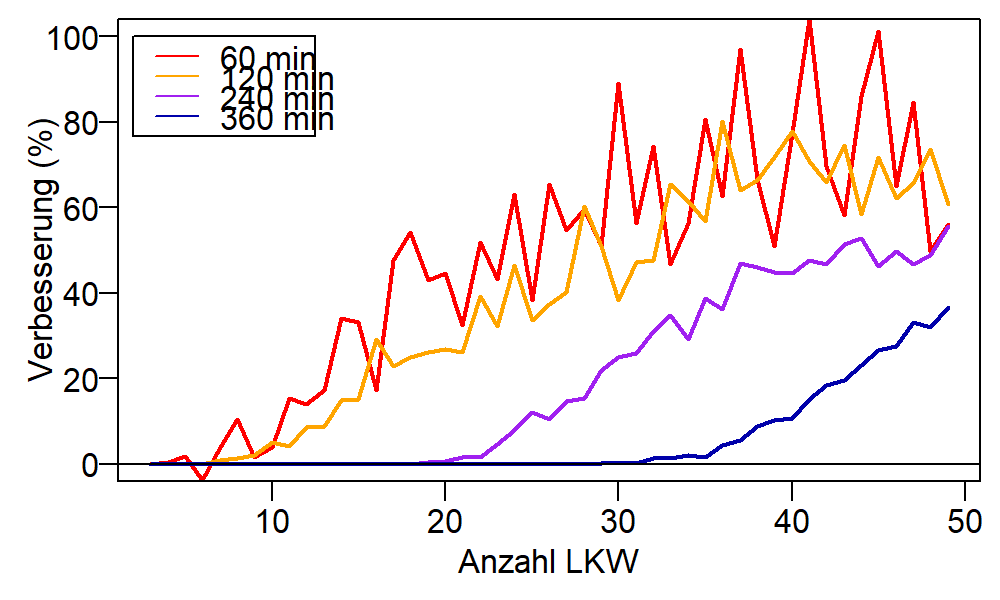
\includegraphics[width=0.7\textwidth]{images/graphs/tspSimALimSlotsize.png}
    \caption{Verhalten bei unterschiedlicher Slotgröße (test3LoadersBestOf50LimitedSlotsize(), tspSlotsize.R)}
    \label{fig:tspEvalSlotsize}
\end{figure}

\todo{Evtl. bis 100 LKW}

Was in dem Auswertungsgraphen zu erkennen ist, ist dass sich die Verbesserung für alle Slotgrößen im Mittel auf maximal 60-70\% Verbesserung einpendelt \todo{Mit längerem Graphen verifizeiren}. Je größer der Slot ist, desto länger dauert dies natürlich, mehr LKW hineinpassen und eine gewisse Überbuchung notwendig ist. So erkennen ist aber auch, dass schon die Durchschnittswerte extrem schwanken, je kleiner der Slot ist. In einigen Fällen lässt sich dort eine sehr gute Verbesserung erzielen, in anderen aber auch eine sehr viel weniger Gute. Erklären lässt sich das vermutlich damit, dass ein kleiner Slot einfach sehr begrenzt ist. Der Spielraum bei der Optimierung ist wesentlich geringer und die \glqq{}Ketten\grqq{} von LKW, welche gleiche oder ähliche Kategorien haben und somit alle nacheinander mit dem gleichen Ladehilfmittel abgefertigt werden können, sind einfach wesentlich kürzer. Es sind zwangsweise mehr Hilfsmittelwechsel, spätestens zum Anfang und Ende des Slots nötig. Aus dieser Betrachtung heraus kann man also sagen, dass größere Slots tendenziell besser sind. Mit einer entsprechend auch höheren Anzahl von Buchungen lassen sich ähnlich hohe Verbesserungen erzielen, deren Höhe ist allerdings wesentlich konstanter und weniger schwankend. Hier ist eine Abwägung zwischen Bedürfnissen des Terminals und der LKW Fahrer nötig.


\textbf{Anzahl von Ladeplätzen}

Ebenfalls ist es interessant, wie sich der Algorithmus verhält, wenn die Zahl der Ladeplätze variiert wird. Auch wenn dies vermutlich kein Parameter ist, auch den die Entwickler einen großen Einfluss haben und der vermutlich vom Terminal vorgegeben ist, so kann es doch zumindest interessant sein, das Verhalten des Algorithmus in dieser Situation zu kennen. Ausgewertet wurde im folgenden die Anzahlen 1, 3, 5 und 10 der Ladeplätze, was einige beispielhafte Werte darstellt, die vermutlich in dieser Größenordnung in der Realität vorkommen.

\begin{figure}[H]
    \centering
    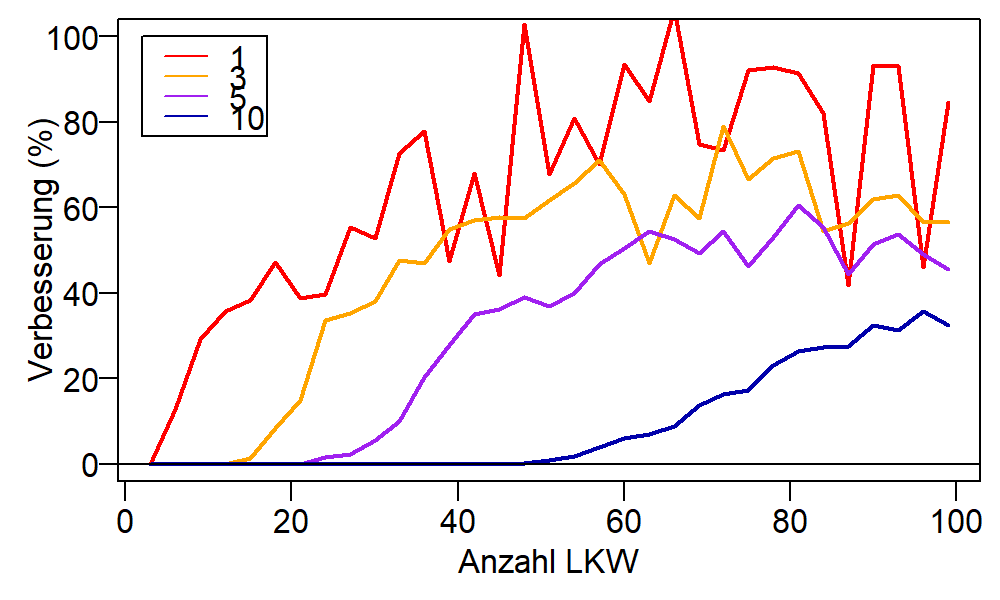
\includegraphics[width=0.7\textwidth]{images/graphs/tspSimALimLoaders.png}
    \caption{Verhalten bei unterschiedlicher Anzahl von Ladeplätzen (test3LoadersBestOf50LimitedLoaders(), tspLoaders.R)}
    \label{fig:tspEvalLoaders}
\end{figure}

Bei der Änderung der Anzahl von Ladeplätzen lassen sich ganz ähnliche Beobachtungen machen, wie auch schon bei Änderung der Slotgröße. Der Anstieg ist bei kleinerer Anhal von Plätzen natürlich zunächst höher, da auch insgesamt weniger LKW hinein passen. Allerdings geht die relative Verbesserung auch hier wieder in ähnlich hohe Regionen. Es ist auch wieder zu erkennen, dass die Schwankung bei wenigen Slots extrem hoch ist und mit steigender Anzahl deutlich geringer wird. Die Durchschnittskurven sind hier deutlich gleichmäßiger. Auch hier dürfte das mit dem Planungsspielraum zusammenhängen, da die Buchungen einfach auf mehr Plätze aufgeteilt werden können und so auf jedem Platz weniger Wechsel zwischen den Ladekategorien und -hilfsmitteln stattfindet. Im Endeffekt sind also auch hier wieder mehr Ladeplätze besser geeignet für eine gleichmäßige Verteilung, auch wenn im allgemeinen Durchschnitt in allen Varianten ähnlich viele LKW bearbeitet werden können.


\textbf{Ungleiche Verteilung der Ladekategorien}



